\documentclass[a4paper, 11pt]{article}
\usepackage{comment}
\usepackage{lipsum}
\usepackage{fullpage}
\usepackage[utf8]{inputenc}
\usepackage[T1]{fontenc}
\usepackage{amsmath}
\usepackage{libertine}
\usepackage{libertinust1math}
\usepackage{listings}
\usepackage{wrapfig}
\usepackage{color}
\usepackage{graphicx}
\graphicspath{ {images/} }


\definecolor{pblue}{rgb}{0.13,0.13,1}
\definecolor{pgreen}{rgb}{0,0.5,0}
\definecolor{pred}{rgb}{0.9,0,0}
\definecolor{pgrey}{rgb}{0.46,0.45,0.48}

\lstset{
    language=java,
    showspaces=false,
    showtabs=false,
    breaklines=true,
    showstringspaces=false,
    breakatwhitespace=true,
    commentstyle=\color{pgreen},
    keywordstyle=\color{pblue},
    stringstyle=\color{pred},
    basicstyle=\tiny,
    moredelim=[il][\textcolor{pgrey}]{$$},
    moredelim=[is][\textcolor{pgrey}]{\%\%}{\%\%}
}



\begin{document}

\noindent
\large\textbf{Algorithmen und Datenstrukturen} \hfill \textbf{Christoph Stach (555912)} \\
\normalsize Aufgabe 2: Einfach und doppelt verkette Liste \hfill Tom Buhrtz \\

\section*{Erarbeiten Sie sich die notwendige Datenstruktur einer einfach verketteten Liste}


\subsection*{SinglyLinkedList}
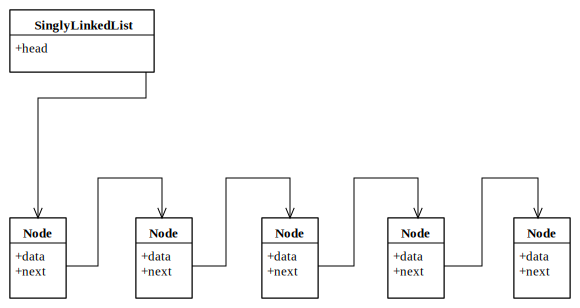
\includegraphics[width=\linewidth]{SinglyLinkedList}
\subsection*{DoublyLinkedList}
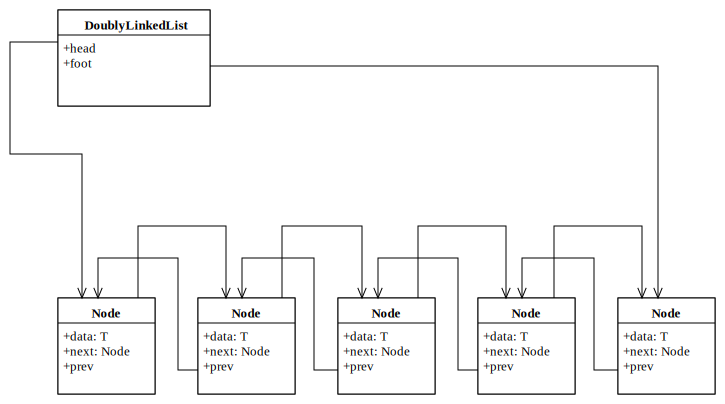
\includegraphics[width=\linewidth]{DoublyLinkedList}


\section*{Zu speichern in unserer Liste sind Studenten mit Vor- und Nachnamen nebst Matrikelnummer und Studiengang.
          Entwerfen Sie die notwendigen Datentypen und begründen Sie gegebenenfalls Ihre Wahl.}


\begin{center}
    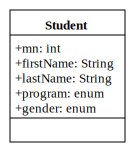
\includegraphics[width=0.5\linewidth]{Student}
\end{center}

\begin{itemize}
    \item int mn: Kann ein Integer sein, da es sich um ganze Zahlen handelt
    \item String firstName: Ein String, da Zeichenketten gespeichert werden müssen
    \item String lastName: Ein String, da Zeichenketten gespeichert werden müssen
    \item Program program: Ein Enum ist Performater zu sortieren als Strings (intern sind Enums Integer) und in der implementierung eleganter.
Das Enum enthält die entsprechende Studiengänge z.B. APPLIED\_COMPUTER\_SIENCE
    \item Gender gender: Ein Enum ist Performater zu sortieren als Strings (intern sind Enums Integer) und in der implementierung eleganter.
Das Enum enthält entsprechen FEMALE und MALE
\end{itemize}

\pagebreak

\section*{Einige Methoden obiger einfach verketteter Liste lassen sich (im Gegensatz zum
          Array oder einer doppelt verketteten Liste) effizient (in unterschiedlicher Hinsicht)
          implementieren, andere nicht unbedingt - welche sind das und warum?}

\subsection*{insertFirst()}
Die Methode lässt sich bei der einfach und doppelt verketteten Liste sehr leicht implementieren, da nur ein neuer Kopf
gesetzt werden muss. Im Vergleich zum Array muss hier weniger Aufwand geleistet werden, da ein Array komplett neu
erstellt werden müsste um den neuen Wert zu speichern.

\subsection*{insertLast()}

Ähnlich wie bei \textit{insertFirst()} kann bei der doppelt verketteten Liste einfach ein neuer Fuß gesetzt werden, was
sehr einfach ist, da die doppelt verkette Liste bereits eine Referenz auf den Fuß hat. Bei bei der einfach verketteten
Liste gestaltet sich das komplizierter, weil erst die komplette Liste durchlaufen werden muss um den Fuß zu finden.
Das Array müsste wieder neu erstellt werden.

\subsection*{insert()}

Um Elemente einzufügen müssen beide Listen jeweils bis zum Index durchlaufen werden. Hier können sich die Vorteile einer
doppelt verketten Liste zu nutze gemacht werden, da bei einem Index der größer ist als die Hälfe der Länge der Liste auch
von hinten angefangen werden kann die Liste zu durch laufen. Die implementierung ist dadurch natürlich komplexer aber
man hat unter Umständen im Vergleich zur einfach verketteten Liste Performancevorteile. Das Array müsste wieder neu
erstellt werden.


\subsection*{remove()}
Wie bei \textit{insert()} müssen die Listen wieder zum Index durchlaufen werden. Das Element wird entfernt in dem man
Beim Vorgänger Element die \textit{next} Eigenschaft anpasst. Bei der Doppelt verketteten Liste muss zusätzlich auch
noch die \textit{prev} Eigenschaft angepasst werden. Das zu entfernende Element wird gefunden in dem man wieder bis zum
jeweiligen Index durchläuft. Bei der Doppelt verketteten Liste kann sich unter Umständen die Eigenschaft zu nutze
gemacht werden das man von Hinten anfangen kann die Liste zu durchlaufen um das Element zu finden.

\subsection*{get()}
Das finden des jeweiligen Elements funktioniert gleich wie bei \textit{insert()} und \textit{remove()}.
Die Doppelt verkette Liste bietet die gleichen Vorteile wie sonst.

\subsection*{size()}
Die Methode lässt sich sehr einfach implementieren da nur der Wert der Instanzeigenschaft \textit{size} zurückgeben
werden muss. Ein Array hat dafür die native Eigenschaft \textit{.length}.

\subsection*{empty()}
Lässt sich bei den Listen auch sehr einfach implementieren da nur überprüft werden muss ob der Kopf == \textit{null} ist.
Alternativ kann auch überpüft werden ob die \textit{size} == \textit{0} ist.

\subsection*{clearAll()}
Die Methode ist einfach und Performant bei beiden Listen zu implementieren. Bei der einfach verketten Liste muss der
Kopf auf \textit{null} gesetzt werden. Außerdem muss die Instanzeigenschaft \textit{size} auf \textit{0} gesetzt werden.
Bei der doppelt verketten Liste muss zusätzlich der Fuß auf \textit{null} gesetzt werden. Ein Array müsste nur mit einem
neuen Array der Länge \textit{0} bzw. mit \textit{null} inititialisiert werden.


\subsection*{Zusammenfassung}
Im Allgemeinen kann man sagen das Listen das schreibenden Methode bei Listen wie \textit{insert()}, \\
\textit{insertFirst()}, \textit{insertLast()} und \textit{remove()} besser implementiert sind im gegensatz zum Array
besser implementiert werden können. Das Array muss bei schreibenen Methoden jedes mal komplett neu aufgebaut und die
Elemente müssen in das neue Array kopiert werden. Um die Länge korrekt ermitteln zu können müssen bei den Listen die
Methoden \textit{insert()}, \textit{insertFirst()}, \textit{insertLast()} und \textit{remove()}  die Instanzeigenschaft
\textit{size} jeweils um \textit{1} hochzählen bzw. verringern. Beim Array kann die Länge direkt nativ gelesen werden.

\section*{Analysieren Sie die Komplexität der von ihnen implementierten Sortierverfahren
          allgemein und im speziellen Fall Ihrer Implementierung}

\subsubsection*{Bubble Sort}

\begin{lstlisting}[language=java]
void sort(Listable<T> listable, Comparable<T> comparable) {
    boolean swapped;                                    //
    int i = 1;                                          // | 1
                                                        //
    do  {                                               //              |
        swapped = false;                                // | 2          |
        for (int j = 0; j < listable.size() - i; j++) { // | 2      |   |
            if (comparable.compare(listable.get(j),     //          |   |
                listable.get(j + 1)) > 0) {             // | 2x+3   |   |
                                                        //          |   |
                swap(listable, j, j + 1);               // | 3x+y+1 | n | n
                swapped = true;                         // | 1      |   |
            }                                           //          |   |
        }                                               //          |   |
                                                        //              |
        i++;                                            // | 1          |
    } while (swapped);                                  //              |
}

void swap(Listable<T> listable, int a, int b) {         //       |
    T memorizedObject = listable.get(a);                // | x+y |
    listable.set(a, listable.get(b));                   // | y   | 3x+y
    listable.set(b, memorizedObject);                   // | y   |
}                                                       //       |
\end{lstlisting}
x = Laufzeit von listable.get() \\
y = Laufzeit von listable.set() \\
n = Anzahl Datensätze \\
\ \\
\( T(n, x, y) = 1 + n(2 + n(2 + 2x + 3 + 3x + y + 1 + 1) + 1) \) \\
\( T(n, x, y) = 1 + n(3 + n(5x + y + 7)) \) \\
\( T(n, x, y) = 1 + n(3 + 5nx + ny + 7n) \) \\
\( T(n, x, y) = 1 + 3n + 5n^2x + n^2y + 7n^2 \) \\
\ \\
Schlechtester Fall:      \( O(n^2) \) \\
Bester Fall:             \( O(n) \)   \\
Durschnitt:              \( O(n^2) \) \\

\pagebreak

\subsubsection*{Quick Sort}

\begin{lstlisting}[language=java]
public void sort(Listable<T> listable, Comparable<T> comparable) {
    quickSort(listable, comparable,                          //
        0, listable.size() - 1);                             // | 1
}

private void quickSort(Listable<T> listable,
    Comparable<T> comparable, int from, int to) {                                              |
                                                                                               |
    if (from < to) {                                         // | 1                            |
        int pivotIndex = sortFromTo(listable,                //                                |
            comparable, from, to);                           // | 2+x+1+n(1+x+2+3x+y+1+1)+3x+y |
                                                             //                                |
        quickSort(listable, comparable,                      //                                | log(n)
            from, pivotIndex - 1);                           // | 1                            |
        quickSort(listable, comparable,                      //                                |
            pivotIndex + 1, to);                             //                                |
    }                                                        // | 1                            |
}                                                                                              |

private int sortFromTo(Listable<T> listable,
    Comparable<T> comparable, int from, int to) { // = 2+x+1+n(1+x+2+3x+y+1+1)+3x+y

    int i = from, j = to - 1;                                 // | 2
    T pivot = listable.get(to);                               // | x+1
                                                              //
    while (i <= j) {                                          // | 1    |
        if (comparable.compare(listable.get(i), pivot) > 0) { // | x+2  |
            swap(listable, i, j);                             // | 3x+y |
            j--;                                              // | 1    | n
        } else {                                              //        |
            i++;                                              // | 1    |
        }                                                     //        |
    }                                                         //        |
                                                              //
    swap(listable, i, to);                                    // | 3x+y
                                                              //
    return i;                                                 //
}

void swap(Listable<T> listable, int a, int b) {               //       |
    T memorizedObject = listable.get(a);                      // | x+y |
    listable.set(a, listable.get(b));                         // | y   | 3x+y
    listable.set(b, memorizedObject);                         // | y   |
}
\end{lstlisting}
x = Laufzeit von listable.get() \\
y = Laufzeit von listable.set() \\
n = Anzahl Datensätze \\
\ \\
\( T(n, x, y) = 1 + ( \log(n) * (1 + 2 + x + 1 + n(1 + x + 2 + 3x + y + 1 + 1) + 3x + y + 1 + 1)) \) \\
\( T(n, x, y) = 1 + ( \log(n) * (6 + x + n(5 + 4x + y) + 3x + y)) \) \\
\( T(n, x, y) = 1 + ( \log(n) * (6 + 4x + 5n + 4nx + ny + y)) \) \\
\( T(n, x, y) = 1 + ( \log(n) * (5n + 4nx + 4x + ny + y + 6)) \) \\
\ \\
Schlechtester Fall:      \( O(n^2) \) \\
Bester Fall:             \( O(n * \log(n)) \) \\
Durschnitt:              \( O(n * \log(n)) \) \\

\end{document}
